\documentclass[11pt,oneside,article]{memoir}

\usepackage[paperwidth=8.5in,paperheight=11in,text={5.8in,9in},centering]{geometry}%\usepackage[usenames,dvipsnames]{xcolor}
\usepackage{amsmath,amssymb}
\usepackage{xcolor}
\usepackage[bookmarks=true,colorlinks=true, linkcolor=blue!40!black, urlcolor=blue!60!black, citecolor=red!50!black]{hyperref}
\usepackage{tabularx}
\usepackage{multirow}
\usepackage{makecell}
\usepackage{tikz}
\usetikzlibrary{decorations.markings,arrows.meta,calc,fit,quotes,cd,positioning}

\tikzset{
   oriented WD/.style={%everything after equals replaces "oriented WD" in key.
      every to/.style={out=0,in=180,draw},
      label/.style={
         font=\everymath\expandafter{\the\everymath\scriptstyle},
         inner sep=0pt,
         node distance=2pt and -2pt},
      semithick,
      node distance=1 and 1,
      decoration={markings, mark=at position .5 with {\arrow{stealth};}},
      ar/.style={postaction={decorate}},
      execute at begin picture={\tikzset{
         x=\bbx, y=\bby,
         every fit/.style={inner xsep=\bbx, inner ysep=\bby}}}
      },
   bbx/.store in=\bbx,
   bbx = 1.5cm,
   bby/.store in=\bby,
   bby = 1.75ex,
   bb port sep/.store in=\bbportsep,
   bb port sep=2,
   % bb wire sep/.store in=\bbwiresep,
   % bb wire sep=1.75ex,
   bb port length/.store in=\bbportlen,
   bb port length=4pt,
   bb min width/.store in=\bbminwidth,
   bb min width=1cm,
   bb rounded corners/.store in=\bbcorners,
   bb rounded corners=2pt,
   bb small/.style={bb port sep=1, bb port length=2.5pt, bbx=.4cm, bb min width=.4cm, bby=.7ex},
   bb/.code 2 args={%When you see this key, run the code below:
      \pgfmathsetlengthmacro{\bbheight}{\bbportsep * (max(#1,#2)+1) * \bby}
      \pgfkeysalso{draw,minimum height=\bbheight,minimum width=\bbminwidth,outer sep=0pt,
         rounded corners=\bbcorners,thick,
         prefix after command={\pgfextra{\let\fixname\tikzlastnode}},
         append after command={\pgfextra{\draw
            \ifnum #1=0{} \else foreach \i in {1,...,#1} {
               ($(\fixname.north west)!{\i/(#1+1)}!(\fixname.south west)$) +(-\bbportlen,0) coordinate (\fixname_in\i) -- +(\bbportlen,0) coordinate (\fixname_in\i')}\fi %Define the endpoints of tickmarks
            \ifnum #2=0{} \else foreach \i in {1,...,#2} {
               ($(\fixname.north east)!{\i/(#2+1)}!(\fixname.south east)$) +(-\bbportlen,0) coordinate (\fixname_out\i') -- +(\bbportlen,0) coordinate (\fixname_out\i)}\fi;
         }}}
   },
   bb name/.style={append after command={\pgfextra{\node[anchor=north] at (\fixname.north) {#1};}}}
}

\newcommand{\pgfextractangle}[3]{
	\pgfmathanglebetweenpoints
		{\pgfpointanchor{#2}{center}}
		{\pgfpointanchor{#3}{center}}
    \global\let#1\pgfmathresult  
}

\newcommand{\pgfportangle}[2]{
	\pgfextractangle{#1}{#2}{#2'}
}

\newcommand{\portdot}[3][]{
	\pgfportangle{\angleout}{#2}
	\draw (#2) to[out=180+\angleout,in looseness=0, #1] (#3.center)                              
}

\newcommand{\portxdot}[3][]{
	\pgfportangle{\angleout}{#2}
	\draw (#2') to[out=\angleout,in looseness=0, #1] (#3.center)                              
}

\newcommand{\portxportx}[3][]{
	\pgfportangle{\angleout}{#2}
	\pgfportangle{\anglein}{#3}
	\draw (#2') to[out=\angleout, in=\anglein, #1] (#3')
}

\newcommand{\portportx}[3][]{
	\pgfportangle{\angleout}{#2}
	\pgfportangle{\anglein}{#3}
	\draw (#2) to[out=180+\angleout, in=\anglein, #1] (#3')
}

\newcommand{\portxport}[3][]{
	\pgfportangle{\angleout}{#2}
	\pgfportangle{\anglein}{#3}
	\draw (#2') to[out=\angleout, in=180+\anglein, #1] (#2)
}

\newcommand{\portport}[3][]{
	\pgfportangle{\angleout}{#2}
	\pgfportangle{\anglein}{#3}
	\draw (#2) to[out=180+\angleout, in=180+\anglein, #1] (#3)
}

\tikzset{
	unoriented WD/.style={
		min rad/.store in=\minrad,
		min rad=.3cm,
		port length/.store in=\portlen,
		port length = .1cm,
		every fit/.style={inner sep=.3cm}
	},
		port label/.style={append after command={\pgfextra{
			\begin{pgfinterruptpath}
				\ifnum \numports=0 {} \else \draw foreach\counter in {1,...,\numports}{
					\pgfextra{\pgfportangle{\angle}{\fixname_port\counter}}
					(\fixname_port\counter) +(\angle+110:8pt)
					node {\scriptsize $#1^{\counter}$}
				};\fi
			\end{pgfinterruptpath}
		}}},
	cell/.style 2 args={%When you see this key, run the code below:
		draw,
		circle,
		minimum size=2*\minrad,
		outer sep=0pt,
		inner sep = .15cm,
		thick,
		prefix after command={\pgfextra{
			\let\fixname\tikzlastnode
			\def\numports{#1}
		}},
		append after command={\pgfextra{
			\begin{pgfinterruptpath}
				\ifnum #1=0{} \else \draw foreach \counter in {1,...,#1}{
					let \n1={(\counter-1)*360/#1+#2} in 
					($(\fixname.\n1)!\portlen!(\fixname.center)$) coordinate (\fixname_port\counter')
					-- ($(\fixname.\n1)!-\portlen!(\fixname.center)$) coordinate (\fixname_port\counter)
				};\fi
			\end{pgfinterruptpath}
		}}
	},
	cell name/.style={append after command={node[anchor=north] at (\fixname.north) {#1}}},
	dot/.style={circle,minimum size=4pt, inner sep=0, fill},
	dot name/.style 2 args={append after command={
		\pgfextra{\node at ($(\tikzlastnode.center)+#1$) {\scriptsize #2};
		}
	}}
}


\def\bhline{\Xhline{2\arrayrulewidth}}
\def\bbhline{\Xhline{2.5\arrayrulewidth}}
\def\bbbhline{\Xhline{3\arrayrulewidth}}

\newcommand{\tn}[1]{\textnormal{#1}}
\def\mcC{\mathcal C}\def\mcD{\mathcal D}
\def\taking{\colon}
\def\Set{\mathsf{Set}}
\def\Hom{\tn{Hom}}
\def\Cat{\mathsf{Cat}}
\def\End{\mathsf{End}}
\def\S{\mathcal{S}}
\newcommand{\set}{\tn{--Set}}

\begin{document}

\author{David I. Spivak}

\title{Final report for Office of Naval Research Grant N000141310260}

\maketitle

This report will summarize my progress toward the goals of ONR grant N000141310260 (``Categorical Informatics"), which was in effect from 2013/02/01 to 2015/10/31. Throughout this period I have been employed by the Department of Mathematics at the Massachusetts Institute of Technology (MIT). Until March 2013 I was a Postdoctoral Associate, under the guidance of Professor Haynes Miller, and in March 2013 I was promoted to the position of  Research Scientist. The Technical Proposal for this grant can be found online at: \url{http://math.mit.edu/~dspivak/informatics/technical_proposal2013.pdf}.

\tableofcontents

\chapter{Research resulting from this grant}

My goals for this grant are discussed in Section I.3 of the \href{http://math.mit.edu/~dspivak/informatics/grants/technical_proposalONR--2013.pdf}{Technical Proposal}. I will summarize them in a list below, and in the subsequent sections I will discuss the degree to which I was able to accomplish each of them. My stated goals for this grant were to:
\begin{itemize}
\item Formalize a notion of hierarchy in information-bearing structures.
\item Develop the theory of updates in databases.
\item Extend previous work on the use of monads in databases.
\end{itemize}
I will discuss each of these in turn below, and then I will also discuss some other accomplishments I made during the project period.

\section{Hierarchy in information-bearing structures}\label{sec:hierarchy}

Formalizing the uses of hierarchy, as found in query languages, dynamical systems, and protein materials has constituted a major part of my effort while working on this grant. The categorical tool that turned out to be most relevant was that of operads, which are categories whose morphisms are many-input, one-output. In this context, a morphism is an arrangement for building one thing---a relation, a dynamical system, a protein---as a combination of many smaller things of the same sort. 

\begin{center}
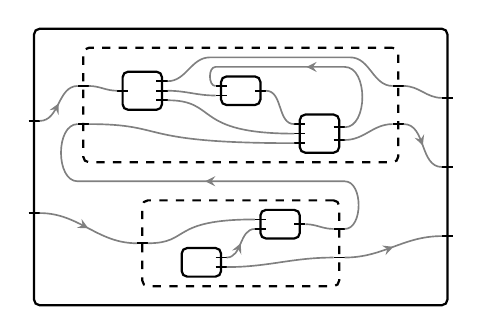
\begin{tikzpicture}[oriented WD, bbx = .5cm, bby =.8ex, bb min width=.5cm, bb port length=2pt, bb port sep=1]
  \node[bb={1}{3}] (X11) {};
  \node[bb={2}{1}, right=1.5 of X11] (X12) {};
  \node[bb={3}{2}, below right=of X12] (X13) {};
  \node[bb={2}{2}, fit={(X11) (X12) (X13) ($(X12.north)+(0,2)$) ($(X13.east)+(.5,0)$)}, dashed] (Y1) {};
  \node[bb={2}{1}, below left=6 and 0 of X13] (X21) {};
  \node[bb={0}{2},below left=of X21] (X22) {};
  \node[bb={1}{2}, fit=(X21) (X22), dashed] (Y2) {};
  \node[bb={2}{3}, fit={($(Y1.north)+(0,1)$) ($(Y2.south)-(0,1)$) ($(Y1.west)-(.25,0)$) ($(Y1.east)+(.25,0)$)}] (Z) {};
  \begin{scope}[gray]
  \draw[ar] (Z_in1') to (Y1_in1);
  \draw[ar] (Z_in2') to (Y2_in1);
  \draw (Y2_in1') to[in looseness=2] (X21_in1);
  \draw[ar] (X22_out1) to (X21_in2);
  \draw (X22_out2) to (Y2_out2');
  \draw[ar] (Y2_out2) to (Z_out3');
  \draw (Y1_in1') to (X11_in1);
  \draw (X13_out2) to (Y1_out2');
  \draw (Y1_in2') to[in looseness=2] (X13_in3);
  \draw (X11_out3) to[in looseness=2] (X13_in2);%
  \draw (X12_out1) to (X13_in1);
  \draw (X11_out2) to (X12_in2);
  \draw (Y1_out1) to (Z_out1');
  \draw[ar] (Y1_out2) to (Z_out2');
  \draw (X21_out1) to (Y2_out1');
  \draw[ar] let \p1=(Y2.north east), \p2=(Y1.south west), \n1={\y1+2*\bby}, \n2=\bbportlen in
  	(Y2_out1) to[in=0] (\x1+\n2,\n1) -- (\x2-\n2,\n1) to[out=180] (Y1_in2);
  \draw[ar] let \p1=(X13.north east), \p2=(X12.north west), \n1={\y2+\bby}, \n2=\bbportlen in
  	(X13_out1) to[in=0] (\x1+\n2,\n1) -- (\x2-\n2,\n1) to[out=180] (X12_in1);
  \draw let \p1=(X12.north west), \p2=(X13.north east), \n1={\y1+2*\bby}, \n2=\bbportlen in
  	(X11_out1) to (\x1-2*\n2,\n1) -- (\x2+2*\n2,\n1) to[out=0] (Y1_out1');
  \end{scope}
  \end{tikzpicture}
\end{center}

In the operadic approach to relational algebra, the boxes correspond to table types---i.e., a set of $n$ columns and their types---drawn as a box with $n$ ports, each labeled with its type. A query is a wiring together of such boxes inside of a larger box. Connecting different tables along common columns corresponds to a categorical limit (or JOIN operation), and the outer box represents a final projection (or SELECT clause). The same idea works for dynamical systems (both discrete and continuous). The different semantics correspond to different \emph{algebras} on the same operad. 

In the technical proposal for this grant, I also outlined an approach to aggregation using what I called Hierarchical Categories. This approach did not seem to bear fruit. Recently, however, my colleague Ryan Wisnesky came up with nearly the same model independently while trying to formalize the Nested Relational Calculus, an important style of databases used in XML and JSON. It may be that with his help, the hierarchical category idea will play a role in future work.

\section{Theory of updates}

Database updates are commands issues by a user, which take any state and produce a new one. For example, inserting the record (Barack, Obama, 1961) is something that can be done regardless of the current state. Similarly, deleting this record is an update, so it can be done regardless of state; however, note that this update will have no effect if the state does not currently contain this record. Thus database updates are usually conceived of as functions from the set of possible states to itself. In the category-theoretic setting, one can ask whether updates are in fact \emph{functorial}, and they are. Given a database homomorphism between two states, there is an induced database homomorphisms between their updates. This is true not only for insert and delete updates, but also modify-in-place updates, such as changing Robert to Bob, or increasing everyone's salary by 5\%. 

Certain updates come with additional structure. For example, if $U$ is an insert update, then for any state $S$, there is an induced database homomorphism $S\to U(S)$. This is a natural transformation from the identity functor to the update functor. De-duplication updates also come with such a map $S\to D(S)$. On the other hand, if $V$ is a delete update, there is a natural map $V(S)\to S$. The existence of such natural maps has led some categorical database researchers, such as Rosebrugh and Johnson, to consider updates as database homomorphisms, $S\to S'$, but I believe this misses the idea that updates are commands issued independently of state. That said, their work on the view-update problem seems to be workable even in the update-as-functor setting, after just a bit of reworking. 

There is a very large category (in a technical sense) of functors $C\set\to C\set$, whereas there is a syntax for, and therefore a countable number of, updates used in practice. Finding a smaller class of updates that is closed under composition is thus an important issue. It appears that the class of polynomial endofunctors $P\colon C\set\to C\set$ serves in this capacity. Polynomial functors are precisely what we use to capture data migration functors, including ETL processes. It turns out that queries are a particular case (in which we migrate data from our database to a one-table database). We now see updates as another special case, in which we migrate data from our database to itself. This means that queries, updates, and ETL processes all take a common, and composable form. 


\section{Use of monads in databases}

Monads can be used to relax the atomicity constraint for relational databases. More precisely, given any monad $T$ on the category of sets, one can consider its Kleisli category $\Set_T$, and define the category of $T$-states on a database schema $C$ to be the category of functors $C\to\Set_T$. For example, using the powerset monad $T$, the foreign key columns of a database are filled with sets of IDs from other tables, rather than atomic elements. This is reminiscent of the nested relational calculus, which is based entirely on the powerset monad. As a much more basic instance of this idea, consider the case of \emph{nullable columns}, which are columns in which a value can be NULL. This corresponds to the so-called "maybe" or "option" monad, namely the functor $X\mapsto X+1$.

In a paper called "Kleisli database instances", I discuss the above idea to use monads in databases. What that paper missed is that different columns should be using different monads. Some columns require atomic data, some allow nullable data, some could allow subsets or probability distributions or general linear combinations of data, etc. It was unclear how to include all this structure. I now understand this much better, as I will discuss below. However, I also realize that by adding so much expressivity, much is lost. For example, instead of having three data migration functors emerge for any functor $F\colon C\to D$ between schemas, there is only one in the above framework. Thus it remains unclear whether this model is viable, especially for information integration tasks.

Let $\End$ be the category of finitary endofunctors on $\Set$, a category which includes the finitary monads. We can consider $\End$ as a 2-category with one object. There is an 2-embedding $i\colon \End\to\Cat$, sending the unique object to the category $\Set$. Let $\S=\int i$ be the Grothendieck construction applied to this functor. An object in $\S$ is just a set. A morphism $X\to Y$ in $\S$ consists of a finitary endofunctor $T$ together a function $X\to T(Y)$. For example, a function $X\to Y+1$ is a morphism over the maybe monad. Define a schema in this setting to be a 2-category $C$ over $\End$, so that each morphism is labeled with a monad. An instance on $C$ is then a 2-functor $C\to\S$ over $\End$. 

While one data migration functor, pullback along $F\colon C\to D$ does exist, it does not have a left or right adjoint. One way to see this is that the category $\S$ does not have an initial or terminal object. Indeed, if $\emptyset$ is the empty set, we have an isomorphism of categories $\Hom(\emptyset, X)\cong \End$, for any set $X$. 

\section{Other database research}

We have done a good deal of database research that is outside the scope envisioned at the outset of this grant, but which is certainly part of the major thrust of that research agenda. Patrick Schultz and I have discovered a way to much more tightly link a database and an existing programming language. We are currently writing a paper about this, and in the meantime have worked with Ryan Wisnesky to implement the ideas in working code. Wisnesky has a prototype version working, called \href{http://categoricaldata.net/fql.html}{\tn{FQL}}, in which databases are linked with a Javascript back-end, which can perform arbitrary computations on the data. Queries on such a system are outside the scope of standard SQL and are much more general than database theorists seem to have worked with previously. 

We have also used FQL to integrate not only databases but ontologies. Working with researchers from NIST, we went through an example of a supply chain database that was enriched with an OWL ontology, that included a taxonomy of materials. For example, a query for "machines that can drill a 1-inch hole in any kind of steel" should return results for machines that can drill a 1-inch hole in any kind of metal. We were able to capture all this within FQL, and the query results matched NIST's prior published results. This means that instead of stringing together two different tools (database and ontology), FQL could accomplish the same result alone.

Working with some international colleagues, I was able to salvage an old model of databases, called simplicial databases, using a modern logical formulation. The result was a conference paper called Type theoretical databases.

I also formulated SPARQL graph pattern queries, which are often used in with semantic web technologies, using a classical category-theoretic approach called lifting problems. Later, working with Ryan Wisnesky, I realized that graph pattern queries could also be recast as embedded dependencies, which are an important class of constraints used in database research. It turns out that the database technique, called the chase, for repairing non-conforming database states corresponds closely with Daniel Quillen's small object argument. We plan to use this observation to establish more principled variants of the chase procedure, by leveraging Richard Garner's recent work on an algebraic small object argument.

\section{Other work}

In Section~\ref{sec:hierarchy}, I mentioned that much of the recent work in my lab has been centered around operads. This has been quite fruitful, leading to a number of papers and several successful grant applications. While I consider only the first of these papers---the one that deals with the relational algebra---to be directly related to the ONR grant, they all have their roots there. This work has also led to a new theorem in rewriting theory, which was discovered jointly with Jason Morton.

I, together with Ravi Jagadeesan, Tristan Giesa, and Markus Buehler, also used operads to produce open-source python software that will construct hierarchical protein materials for use in a molecular dynamics simulator, such as GROMACS or LAMMPS. I have worked a great deal with Buehler's group in the past, resulting in several published articles, but I think this may be our most important contribution to date.

Finally, I worked with Jason Gross and Adam Chlipala to implement a category theory library in Coq, the computer proof assistant. The mathematics is quite layered, and as a result Coq had quite some difficulty handling the complexity. We wrote a paper about how to reduce the burden and make the library more performant.

\chapter{Publications and presentations}

Below I will list some publications, presentations, collaborations, and outreach I have been involved with in connection with the ONR grant.

\section{Book}

Spivak, D.I. (2014) {\em Category theory for scientists}. MIT Press. 486 pages

\section{Journal articles, refereed conference papers, and technical reports}
\begin{itemize}

\item Vagner, D.; Spivak, D.I.; Lerman, E. (2015) ``Algebras of Open Dynamical Systems on the Operad of Wiring Diagrams''. Accepted for publication: \emph{Theory and Application of Categories}. Available online \url{http://arxiv.org/abs/1408.1598}.

\item Morton, J.; Spivak, D.I. (2015) ``A operad-based normal form for morphism expressions in a closed compact category". \emph{Higher-dimensional rewriting and applications}, \url{http://hdra15.gforge.inria.fr}.

\item Giesa, T.; Jagadeesan, R.; Spivak, D.I.; Buehler, M.J. (2015) ``Matriarch: a Python library for materials architecture.'' \emph{ACS Biomaterials Science \& Engineering}, \url{http://pubs.acs.org/doi/full/10.1021/acsbiomaterials.5b00251}.

\item Spivak, D.I.; Wisnesky, R. (2015) ``Relational Foundations for Functorial Data Migration.'' \emph{Database programming languages}. Available online: \url{http://arxiv.org/abs/1212.5303}.

\item Brommer D.B.; Giesa T.; Spivak, D.I.; Buehler, M.J. (2015) ``Categorical Prototyping: Incorporating Molecular Mechanisms into 3D printing". \emph{Nanotechnology}, article reference: NANO-108127.

\item Wisnesky, R.; Spivak, D.I.; Schultz, P.; Subrahmanian, E. (2015) ``Functorial data migration: from theory to practice''. \emph{NIST Interagency/Internal Report (NISTIR)}. Available online: \url{http://arxiv.org/abs/1502.05947}.

\item Forssell, H.; Gylterud, H.K.; Spivak, D.I. (2016) ``Type theoretical databases''. \emph{Logical Foundations of Computer Science}. Available online \url{http://arxiv.org/abs/1406.6268}

\item Spivak, D.I. (2014) ``Database queries and constraints via lifting problems.'' \emph{Mathematical structures in computer science}.  Available online: \url{http://arxiv.org/abs/1202.2591}.

\item Gross, J.; Chlipala, A.; Spivak, D.I. (2014) ``Experience Implementing a Performant Category-Theory Library in Coq''. \emph{5th conference on interactive theorem proving (ITP'14)}. Available online: \url{http://arxiv.org/abs/1401.7694}.

\item Spivak, D.I.; Wisnesky, R. (2013) ``A Functorial Query Language''. \emph{Data-Centric Programming workshop (DCP2014)}. Available online: \url{http://research.microsoft.com/en-us/events/dcp2014/wisnesky.pdf}.

\end{itemize}

\section*{Preprints}

\begin{itemize}

\item Spivak, D.I.; Schultz, P.; Rupel, D. (2015) ``String diagrams for traced and compact categories are oriented 1-cobordisms''. \emph{Submitted.} Available online: \url{http://arxiv.org/abs/1508.01069}.

\item P\'erez, M.; Spivak, D.I. (2015) ``Toward formalizing ologs: Linguistic structures, instantiations, and mappings''. \emph{Submitted.} Available online: \url{http://arxiv.org/abs/1503.08326}.

\item Spivak, D.I.; Schultz, P.; Wisnesky, R. (2015) ``A Purely Equational Formalism for Functorial Data Migration''. Available online: \url{http://arxiv.org/abs/1503.03571}.

\item Spivak, D.I. (2015) ``Nesting of dynamic systems and mode-dependent networks''. \emph{Submitted.} Available online: \url{http://arxiv.org/abs/1502.07380}.

\item Spivak, D.I. (2014) ``Categories as mathematical models''. To appear in \emph{Categories for the Working Philosopher}. Available online \url{http://arxiv.org/abs/1409.6067}.

\item Rupel, D.; Spivak, D.I. (2013) ``The operad of temporal wiring diagrams: formalizing a graphical language for discrete-time processes''. \emph{Submitted.} Available online \url{http://arxiv.org/abs/1307.6894}.

\item Spivak, D.I. (2013) ``The operad of wiring diagrams: Formalizing a graphical language for databases, recursion, and plug-and-play circuits.'' Available online: \url{http://arxiv.org/abs/1305.0297}.


\end{itemize}

\section{Invited Presentations}

U. Mass. Boston (Mathematics colloquium) 2015/10/14;\\
NIST (Computational category theory workshop) 2015/09/28;\\
University of Oslo (Department of Informatics) 2015/09/21;\\
\'{E}PFL (8 hour mini-course) 2015/09/14 -- 2015/09/18;\\
MIT (LIDS lunch seminar) 2015/06/26;\\
NIST 2015/06/16;\\
NIST 2015/06/18;\\
Foundational Methods in Computer Science 2015/06/06;\\
Categorical Foundations of Network Theory workshop (ISI Turin) 2015/05/28;\\
U. Pennsylvania (Complex systems seminar) 2015/04/03;\\
Pennsylvania State U. (Applied algebra and network theory seminar) 2015/03/18;\\
MINES ParisTech (International workshop on Design Theory) 2015/01/26;\\
MIT (Programming languages seminar) 2014/04/15;\\
IAS (Bar talk) 2014/03/20;\\
PARC 2014/03/03;\\
Amgen 2014/03/04;\\ 
Oracle 2014/02/28;\\
UIUC (Topology seminar) 2014/02/25;\\
Harvard (PL seminar) 2014/02/19;\\
Carnegie Mellon U. (POP seminar) 2014/01/23;\\
NIST 2013/06/12;\\


\chapter{Collaborations, outreach, and transitions}

In this section, I will discuss some collaborations that I have taken part in over the grant period (Section~\ref{sec:collaborations}), as well as outreach activities I have performed (Section~\ref{sec:outreach}). Finally, I will discuss transitions in Section~\ref{sec:transitions}.

\section{Collaborations}\label{sec:collaborations}

Below is a list of collaborations, other than those with my postdocs, that have successfully led to papers. \\

\noindent\begin{tabular}{p{1.9in}lp{3.4in}}
\textbf{I collaborated with:}&&\textbf{resulting in:}\\\hline
Members of NIST: Al Jones, Spencer Breiner, and Subrahmanian Eswaran
&&
Two information integration papers, to be published as a result technical report.
\\
Henrik Forssell at U. Oslo
&&
A paper with Forssell's graduate student, which has been submitted to a conference in mathematical logic.\\
Dylan Rupel at Northeastern
&&
Two papers on wiring diagram operads, both of which have been submitted.
\\
Markus Buehler's group at MIT Civil and Environmental Engineering
&&
Several papers on categorical applications to materials science and engineering.
\\
Adam Chlipala's group at MIT CSAIL
&&
A conference paper on implementing a performant category theory library in Coq, a proof assistant.
\\
Jason Morton at Penn State
&&
A paper presented at a conference on the theory of rewriting systems.
\\
Rajesh Kasturirangan at MIT Laboratory for Information and Decision Systems.
&&
Work in progress on a modular approach to applying the scientific method at scale.
\\
Dmitry Vagner at Duke and Eugene Lerman at UIUC
&&
A paper on composing continuous dynamical systems, accepted for publication in \emph{Theory and Applications of Categories}.
\\

\end{tabular}

\section{Outreach}\label{sec:outreach}

I am interested in disseminating my research more widely to a variety of audiences. To that end, I have participated in the following outreach activities. \\

\noindent\begin{tabular}{p{1.9in}lp{3.4in}}
\textbf{I was involved with:}&&\textbf{in which I:}\\\hline
Hosting a summer graduate student
&&
In the summers of 2014 and 2015, I hosted a graduate student named Dmitry Vagner from Duke University. Our work together resulted in a paper that has been accepted for publication, as mentioned above.
\\
EPFL (\'{E}cole Polytechnique F\'ed\'eral Lausanne) in Switzerland
&&
Gave a four-day mini-course in applied category theory to a group of about 20 researchers (professors, postdocs, and graduate students), about half of whom were mathematicians and half were from other sciences. 
\\
MIT Undergraduate Research Opportunity Program
&&
I have mentored several undergraduates working to learn and do research in applied category theory.
\\
\end{tabular}

\section{Transitions}\label{sec:transitions}

My former employee, then postdoc, Ryan Wisnesky has started a company, \emph{Categorical Informatics Inc.}, of which I am to be a cofounder. The company will modify the existing open-source FQL code (which is under a BSD license, with the blessing of MIT), to ready it for commercialization.

My work on operads, wiring diagrams, and modular compositionality led to a need for more research than could be done using ONR funds alone. In December 2013, I was awarded a five-year, \$900,000 grant from the Air Force Office of Scientific Research (AFOSR) to study the interaction of agents. In September 2014, I was awarded a three-year \$300,000 grant from the National Aeronautics and Space Administration (NASA) to study distributed systems as they relate to the National Air Space.

\end{document}